
\chapter{Equipamentos}

Nesta seção, descrevemos os equipamentos essenciais para uma equipe em missão de investigação e contenção de assombrações. Esta lista inclui materiais de detecção, monitoramento e exorcismo, fundamentais para lidar com fenômenos sobrenaturais e garantir a segurança da equipe durante a operação.

\section{Equipamentos de Detecção e Monitoramento}

\begin{itemize}
    \item \textbf{Câmeras de Visão Noturna e Térmica}: Dispositivos de captura de imagem que permitem registrar fenômenos invisíveis a olho nu, como variações de temperatura e aparições em condições de baixa luminosidade.

    \item \textbf{Gravadores de Voz (EVP – Electronic Voice Phenomenon)}: Equipamento para captar vozes e sons em frequências inaudíveis, frequentemente associados à presença de entidades sobrenaturais.

    \item \textbf{Medidor de EMF (Campo Eletromagnético)}: Detecta flutuações eletromagnéticas, um indicador comum de presença paranormal em áreas específicas.

    \item \textbf{Sensores de Movimento Infrared}: Colocados em áreas de alta atividade, esses sensores detectam movimentos em locais escuros ou isolados, oferecendo monitoramento adicional.

    \item \textbf{Detector de Flutuação de Temperatura}: Ferramenta de mão para identificar mudanças bruscas de temperatura, uma ocorrência comum durante atividades paranormais.

    \item \textbf{Datalogger}: Dispositivo que monitora e registra dados ambientais (como temperatura, umidade e pressão) ao longo do tempo, permitindo a análise de padrões e anomalias.

    \item \textbf{Câmeras de Vídeo com Visão de 360°}: Dispositivos para monitorar ambientes amplos, permitindo observação em tempo real e gravação de todos os ângulos.

    \item \textbf{Tablets e Notebooks com Software de Análise Paranormal}: Ferramentas digitais para análise de dados coletados, organização de evidências e registro das anotações da equipe.
\end{itemize}

\section{Equipamentos de Exorcismo e Contenção}

\begin{itemize}
    \item \textbf{Água Benta e Frascos para Dispersão}: Pequenos frascos de spray para borrifar água benta em áreas ou objetos possivelmente assombrados.

    \item \textbf{Incenso e Resinas Purificadoras (Sálvia Branca, Mirra e Olíbano)}: Para purificar o ambiente, removendo energias negativas e entidades indesejadas.

    \item \textbf{Sal Consagrado}: Pequenos sacos de sal para criar barreiras de proteção e purificar locais com alta atividade espiritual.

    \item \textbf{Talismãs e Amuletos de Proteção}: Incluem colares, pulseiras e outros objetos sagrados que oferecem proteção aos agentes durante a missão.

    \item \textbf{Crucifixos e Objetos Religiosos}: Utilizados em rituais de exorcismo e banimento, crucifixos de mão e outros símbolos são fundamentais para a segurança espiritual.

    \item \textbf{Velas Pretas e Brancas}: Para rituais de proteção e banimento, específicas para contenção de assombrações e purificação de espaços afetados.

    \item \textbf{Livro de Rituais e Orações}: Contém orações específicas para exorcismo e banimento de espíritos, com instruções adaptadas para diferentes crenças ou tipos de entidade.

    \item \textbf{Cristais de Quartzo e Ametista}: Utilizados para harmonizar e purificar o ambiente, afastando energias negativas.

    \item \textbf{Cordas de Proteção e Símbolos Místicos para Selagem}: Utilizadas para isolar áreas afetadas ou selar portais espirituais caso sejam encontrados durante a investigação.

    \item \textbf{Kit de Combate a Vampiros (Antiguidade)}: kits históricos para combate a vampiros, que por terem sido usados no passado com sucesso possuem poderes reforçados.
\end{itemize}

\begin{figure}[hbt]
    \centering
    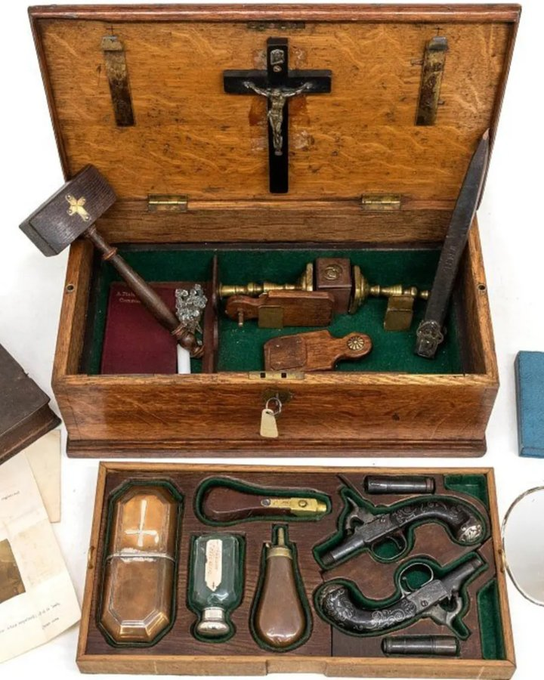
\includegraphics[width=0.5\linewidth]{imagens/VampireKillingSet.png}
    \caption{Caption}
    \label{fig:enter-label}
\end{figure}

\section{Itens Diversos de Apoio à Missão}

\begin{itemize}
    \item \textbf{Lanternas de Mão com Luz UV}: Para detecção de marcas, rastros ou inscrições ocultas que não são visíveis sob luz normal.

    \item \textbf{Rádio Comunicador de Longo Alcance}: Para manter a comunicação entre a equipe em locais isolados ou durante investigações noturnas.

    \item \textbf{Kit de Primeiros Socorros}: Inclui itens básicos para tratar ferimentos leves, desmaios e outros acidentes que possam ocorrer durante a missão.

    \item \textbf{Registro Digital e Anotação (Gravador de Voz e Canetas Marcadoras)}: Equipamentos para documentar observações e registros em campo.

    \item \textbf{Roupas de Proteção Contra o Frio e Máscaras de Proteção}: Equipamentos apropriados para ambientes úmidos ou com pouca ventilação, comuns em cavernas e túneis.
\end{itemize}

\section{Resumo dos Equipamentos para Missão}

A lista de equipamentos acima cobre as necessidades de uma investigação de assombrações, incluindo proteção espiritual, materiais de detecção e recursos tecnológicos para monitorar e coletar evidências. Com esses itens, a equipe terá recursos para garantir segurança e eficiência, maximizando as chances de sucesso na investigação dos fenômenos sobrenaturais.



